%% Requires compilation with XeLaTeX or LuaLaTeX
\documentclass[10pt,xcolor={table,dvipsnames},t]{beamer}
\usetheme[background=dark]{trigon}
\usepackage{amsmath}
\usepackage{nicefrac}
\usepackage{amssymb}
%\usepackage{enumitem}
\usepackage{braket}
\usepackage{empheq}
\usepackage{color}
\usepackage{keyval}
\usepackage{subcaption}
\usepackage{calrsfs}
\usepackage{hyperref}
\usepackage{eufrak}
\usepackage{transparent}
\usepackage{tikz}
\usepackage{nicematrix}

\captionsetup{font=scriptsize}
\title{Open Quantum System}
\subtitle{
  Lectures: \\ 
  \footnotesize
  \begin{itemize}
      \setlength\itemsep{-0.5em}
    { 
      \transparent{0.4}
    \item[] Last time:
    \item Daniel Manzano, A short introduction to the Lindblad master equation (\textit{all})
    \item Breuer and Petruccione, The Theory of Open Quantum Systems (\textit{ch. 3 - 4.3})
    \item Daniel A. Lidar, Notes on the Theory of Open Quantum Systems (\textit{up to ch. 12})
    }
  \item[] Today:
    \item Buča, B., Tindall, J. \& Jaksch, D. Non-stationary coherent quantum many-body dynamics through dissipation
    \item Victor V. Albert \& Liang Jiang, Symmetries and conserved quantities in Lindblad master equations
    \item Cameron Booker, Berislav Buča, Dieter Jaksch, Non-stationarity and Dissipative Time Crystals: Spectral Properties and Finite-Size Effects
    \item Victor V. Albert. Lindbladians with multiple steady states: 
      theory and applications. A Dissertation Presented to the Faculty of the Graduate School of Yale University
  \end{itemize}
  \vspace{-1cm}
}
\newcommand{\dt}{\frac{d}{dt}}
\newcommand{\lan}{\mathcal{L}}
\newcommand{\Hint}{H_{\text{int}}}
\newcommand{\outerprod}[2]{\ket{#1}\!\!\bra{#2}}
\newcommand{\tr}[2]{\text{Tr}_{#1}\bigl[#2\bigr]}
\newcommand{\kett}[1]{\vert #1 \rangle\!\rangle}
\newcommand{\circledmathfrak}[1]{
  \tikz[baseline=(char.base)]{
    \node[shape=circle,draw,inner sep=2pt] (char) {$\mathfrak{#1}$};
  }
}


\setbeamertemplate{footline}{
  \hbox{%
    \begin{beamercolorbox}[wd=.5\paperwidth,ht=2.5ex,dp=1ex,left]{author in head/foot}%
      %\usebeamerfont{author in head/foot}\insertshortauthor~~(\insertshortinstitute)
    \end{beamercolorbox}%
    \begin{beamercolorbox}[wd=.5\paperwidth,ht=2.5ex,dp=1ex,right]{title in head/foot}%
    \end{beamercolorbox}}%
  \vskip0pt%
}

\newlength\mytemplen
\newsavebox\mytempbox
\usepackage{accents}
\newlength{\dhatheight}

\newcommand{\doublehat}[1]{%
    \settoheight{\dhatheight}{\ensuremath{\hat{#1}}}%
    \addtolength{\dhatheight}{-0.15ex}%
    \hat{\vphantom{\rule{1pt}{\dhatheight}}%
    \smash{\hat{#1}}}}

\newcommand\mybluebox{%
    \@ifnextchar[%]
       {\@mybluebox}%
       {\@mybluebox[0pt]}}

\definecolor{myblue}{rgb}{.8, .8, 1}

\def\@mybluebox[#1]{%
    \@ifnextchar[%]
       {\@@mybluebox[#1]}%
       {\@@mybluebox[#1][0pt]}}

\def\@@mybluebox[#1][#2]#3{
    \sbox\mytempbox{#3}%
    \mytemplen\ht\mytempbox
    \advance\mytemplen #1\relax
    \ht\mytempbox\mytemplen
    \mytemplen\dp\mytempbox
    \advance\mytemplen #2\relax
    \dp\mytempbox\mytemplen
    \colorbox{myblue}{\hspace{1em}\usebox{\mytempbox}\hspace{1em}}}

\begin{document}

\begin{frame}
  \titlepage
\end{frame}

\begin{frame}{Dynamical symmetries}
  \only<1->{
  \begin{block}{Diagonal Lindblad}
    $$
    \mathcal{L}\rho = - i[H_S + H_{LS}, \rho] + \sum_{\mu}\biggl(2L_\mu \rho L_\mu^\dag - 
    \bigl\{ L_\mu ^\dag L_\mu, \rho \bigr\} \biggr)
    \quad \text{ with } L_\mu \equiv L_\nu(\omega)
    $$
  \end{block}
}
\only<2->{
  \begin{block}{Dynamical symmetry}
    $$
    \forall \; \mu \equiv (\nu, \omega)\, , \quad \bigl[ \underbrace{L_\mu}_{L_\nu(\omega)}, A \bigr] = 0 
    \qquad \text{ with }\; L_\nu(\omega) \coloneq \sum_{\omega = \epsilon' - \epsilon} \outerprod{\epsilon}{\epsilon}
    L_\nu \outerprod{\epsilon'}{\epsilon'}
    $$
  \end{block}
}
\only<3->{
  \begin{block}{Remembering}
    $$
    \Hint \equiv \sum_\alpha S_\alpha \otimes B_\alpha \quad \text{ and } \quad L_\nu = \sum_{i} u_{i,\nu}S_i
    $$
  \end{block}
}
\end{frame}
\begin{frame}{Dynamical symmetries}
  \begin{block}{Commutator}
  \only<1->{
     Re-writing commutator - $[L_\nu(\omega), A] = 0 \quad \forall \, (\nu, \omega)$\\
   }
   \only<2->{
     Giving for a specific $\omega$ and $\nu$
     \begin{align}
     \Bigl[\sum_{\omega = \epsilon' - \epsilon}\outerprod{\epsilon}{\epsilon}L_\nu \outerprod{\epsilon'}{\epsilon'}
       , A
     \Bigr] = 0 \qquad \forall\,(\nu, \omega)\\
     \Bigl[\sum_{\omega = \epsilon' - \epsilon}\outerprod{\epsilon'}{\epsilon'}L_\nu^\dag \outerprod{\epsilon}{\epsilon}
       , A
     \Bigr] = 0 \qquad \forall\,(\nu, \omega)
   \end{align}
   }
   \vspace{0.5cm}
   \end{block}
   \only<3->{
     \begin{center}
   \textbf{Question: } what can one say on $A$ and/or $L_{\nu}$?
 \end{center}
 }
 
\end{frame}
\begin{frame}{Dynamical symmetries}
  \begin{columns}
    \begin{column}{0.7\textwidth}
      \only<1->{
      \textsl{Assumption $\circledmathfrak{a}$} - for every $\omega$, a unique pair 
      $(\epsilon, \epsilon')$ exists.\\
      \textsl{Note} - assuption \textbf{not} the same as 
      non-degeneracy\\
    }
    \only<2->{
      Then, for a chosen $(\nu, \epsilon)$, one writes
      \begin{align}
     \Bigl[\outerprod{\epsilon}{\epsilon}L_\nu \outerprod{\epsilon'}{\epsilon'}
       , A
     \Bigr] = 0 \qquad \forall\,(\nu, (\epsilon',\epsilon))\\
     \Bigl[\outerprod{\epsilon'}{\epsilon'}L_\nu^\dag \outerprod{\epsilon}{\epsilon}
       , A
     \Bigr] = 0 \qquad \forall\,(\nu, (\epsilon', \epsilon))
   \end{align}
 }
    \end{column}
    \begin{column}{0.3\textwidth}
      \only<1->{
      \vspace{-1cm}
      \begin{figure}
        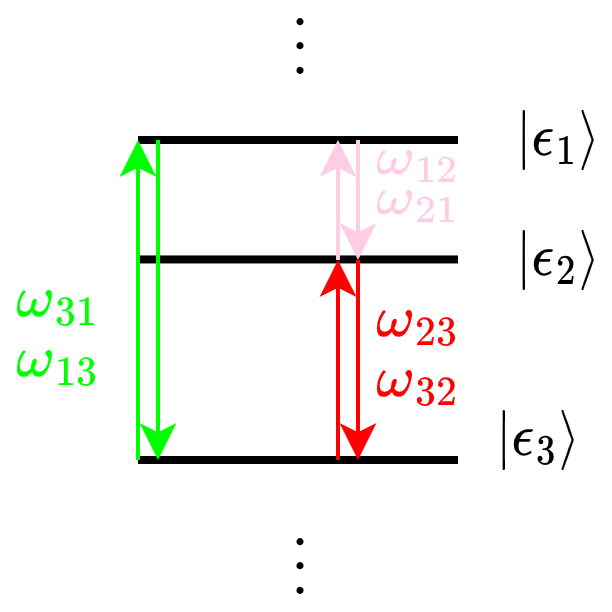
\includegraphics[width=\textwidth]{./energy_levels.png}
      \end{figure}
    }
    \end{column}
  \end{columns}
  \vspace{0.5cm}
  \only<3->{
  The states $\{\ket{\epsilon}\}$ - the chosen orthonormal eigenkets of the Hamiltonian $H_S$.
  Clearly, the ket-bra's span the Liouville space -
  $$
  \mathfrak{D}(\mathcal{H}) = \text{span}(\{\outerprod{\epsilon}{\epsilon'}\}) \quad \forall\,(\nu, (\epsilon',\epsilon))
  $$
}
\end{frame}
\begin{frame}{Assumption $\circledmathfrak{a}$}
  \only<1->{
  Using the completeness relation, 
  $$
  L_\nu = \sum_{\varepsilon, \varepsilon'} \outerprod{\varepsilon}{\varepsilon}L_\nu \outerprod{\varepsilon'}{\varepsilon'}
  $$
  For all $(\nu, (\epsilon, \epsilon'))$, one writes 
}
\only<2->{
  \begin{equation}
    \begin{split}
      L_\nu A - AL_\nu &= \sum_{\varepsilon, \varepsilon'} \outerprod{\varepsilon}{\varepsilon}L_\nu 
  \outerprod{\varepsilon'}{\varepsilon'} A - \sum_{\varepsilon, \varepsilon'} A \outerprod{\varepsilon}{\varepsilon}L_\nu 
  \outerprod{\varepsilon'}{\varepsilon'} \\
                       &= \sum_{\varepsilon}\sum_{\varepsilon'} \underbrace{\Bigl( \outerprod{\varepsilon}{\varepsilon}L_\nu 
  \outerprod{\varepsilon'}{\varepsilon'}A - A\outerprod{\varepsilon}{\varepsilon}L_\nu 
\outerprod{\varepsilon'}{\varepsilon'} \Bigr)}_{0 \text{ for all } (\nu, (\varepsilon, \varepsilon'))} = 0
\end{split}
\end{equation}
}
\only<3->{
The same process can be repeated for $L_\nu^\dag$. \\
Meaning that if such dynamical symmetry exists, 
  $$
  [L_\nu, A] = [L_\nu^\dag, A] = 0
  $$
}
\end{frame}

\begin{frame}{Assumption $\circledmathfrak{a}$}
  \only<1->{
  \begin{center}
  Can one show that $A = \lambda \mathbb{I}$?
\end{center}
}
\only<2->{
  Let the most general form of A:
  $$
  A = \sum_{kl} a_{kl}\outerprod{k}{l}
  $$
}
\only<3->{
  One wants to show that $a_{kl} = 0$ for $k\neq l$. Suppose the contrary - there exists $a_{kl} \neq 0$ for $k\neq l$\\
}
\only<4->{
  Then, the commutator relation will be given by
  \begin{gather}
    \Bigl[\outerprod{m}{m}L_\nu \outerprod{n}{n}, \sum_{kl} a_{kl}\outerprod{k}{l}\Bigr] = 0\\
    \sum_{kl}a_{kl} \outerprod{m}{m}L_\nu \outerprod{n}{n} \outerprod{k}{l} - 
    \sum_{kl}a_{kl} \outerprod{k}{l}\outerprod{m}{m} L_\nu \outerprod{n}{n}
\end{gather}
}
\end{frame}

\begin{frame}{Assumption $\circledmathfrak{a}$}
\only<1->{
  \vspace{-1cm}
  \begin{gather*}
    \sum_{kl}a_{kl} \outerprod{m}{m}L_\nu \outerprod{n}{n} \outerprod{k}{l} - 
    \sum_{kl}a_{kl} \outerprod{k}{l}\outerprod{m}{m} L_\nu \outerprod{n}{n} = \notag \\
    \sum_{l} a_{nl} \outerprod{m}{m} L_\nu \outerprod{n}{l} - \sum_{k} a_{km}\outerprod{k}{m}L_\nu \outerprod{n}{n} \notag \\
\end{gather*}
}
\only<2->{
  \vspace{-1cm}
\begin{gather}
    \xrightarrow[]{\ket{m}} a_{nm}\outerprod{m}{m}L_\nu \ket{n}  = 0 \\
    \xrightarrow[]{\bra{n}} a_{nm} \bra{m}L_\nu \outerprod{n}{n} = 0
\end{gather}
}
\only<3->{
  \vspace{-1cm}
  \begin{itemize}
    \item<3-> Must hold for all $\nu$
    \item<4-> $L_\nu$ was defined to be $\Hint \simeq \sum_\chi L_\chi \otimes B_\chi$, meaning that 
    \item[]<4-> \begin{center} $L_\nu \in \text{span}\bigl( \outerprod{\epsilon}{\epsilon'} \bigr)$\end{center}
    \item<5-> Meaning that $a_{nm} = 0 \; \implies \; \text{contradiction}$
  \end{itemize}
}
\end{frame}

\begin{frame}{Assumption $\circledmathfrak{a}$}
  \only<1->{
  One can show that $A = \lambda \mathbb{I}$, by showing that $a_{jj} = a_{kk} \equiv d_k$. 
}
\only<2->{
  Since $A \sim$  diag.,\\
  $$A = \sum_{k}d_k \outerprod{k}{k}$$
}
\only<3->{
  Using the same expansion, and commutator relations - 
  $$
  d_{\epsilon}\outerprod{\epsilon}{\epsilon} L_\nu \outerprod{\epsilon'}{\epsilon'} - 
  d_{\epsilon'}\outerprod{\epsilon}{\epsilon} L_\nu \outerprod{\epsilon'}{\epsilon'} = 0
  $$
  Meaning that diagonal elements are the same $\implies$
  $$
  A = \lambda \mathbb{I}
  $$
}
\only<4->{
  The newly introduced $\rho_{mn} \coloneq A^n \rho_\infty (A^\dag)^m$ thus do not give any 
  additional imformation. The condition $\mathcal{L}\rho_{mn} = -i(m-n)\lambda \rho_{mn}$
  therefore is redundant.
}
\end{frame}
\begin{frame}{Assumption: continuity}
  \begin{itemize}
    \item<1-> The discrete spectrum: 
      $$
      S_\alpha (\omega) \coloneq \sum_{\omega = \epsilon'-\epsilon} \outerprod{\epsilon}{\epsilon} S_\alpha 
      \outerprod{\epsilon'}{\epsilon'}
      $$
    \item<2-> Continious spectrum: 
      \begin{equation}
        S_\alpha (\omega) = \iint\limits_{\epsilon,\epsilon' \in \sigma(H_S)} \outerprod{\epsilon}{\epsilon}
        S_\alpha \outerprod{\epsilon'}{\epsilon'} \delta\bigl(\omega - (\epsilon - \epsilon') \bigr) d\epsilon\; d\epsilon'
      \end{equation}
  \end{itemize}
\end{frame}

\begin{frame}{Degeneracies?}
  \begin{columns}
    \begin{column}{0.75\textwidth}
      \begin{itemize}
        \item <1-> In addition to the assumption $\circledmathfrak{a}$, one can add degeneracies 
          to the ground level $\ket{d_1}, \ket{d_2}$.
        \item<2-> What does this mean for the commutators?
        \item<2-> Additional terms at $\omega = \epsilon' - \epsilon$ for $0 = \omega = d_1 - d_2$
      \end{itemize}
    \end{column}
    \begin{column}{0.25\textwidth}
      \vspace{-1.0cm}
      \only<1->{
      \begin{figure}
        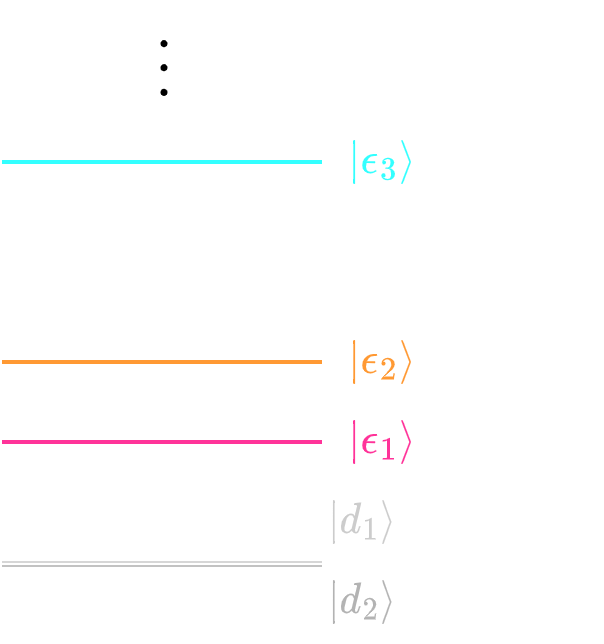
\includegraphics[width=\textwidth]{./energy_levels_deg1.png}
      \end{figure}
    }
    \end{column}
  \end{columns}
  \begin{itemize}
    \item<3->[] 
      \begin{center}
      $\Bigl[ \outerprod{d_1}{d_1}L_\nu \outerprod{d_2}{d_2} + \outerprod{d_2}{d_2}L_\nu \outerprod{d_1}{d_1}, 
      \underbrace{A}_{\equiv a_{ij}} \Bigr] = 0$
    \end{center}
  \item<4->[] Using same procedures as before, one can obtain some relations as for example 
    \begin{center}
      $a_{d_1, d_2}\bra{d_2}L_\nu \ket{d_1} -a_{d_2, d_1} \bra{d_1}L_\nu \ket{d_2} = 0$\\
      $a_{d_1,d_1}\bra{d_2}L_\nu \ket{d_1} - a_{d_2, d_2} \bra{d_2}L_\nu \ket{d_1} = 0$
    \end{center}
  \end{itemize}
\end{frame}
\begin{frame}{Degeneracies}
  \begin{itemize}
    \item<1->[] This suggest the form of $A$ 
      $$
\begin{pNiceArray}{cc|ccc}
  \Block{2-2}<\Large>{\mathbf{A^*_0}}& & \ddots & * & \ddots \\
                                    && * & \ddots & * \\
  \hline
  \ddots & * & \Block{3-3}<\Large>{\mathbf{\lambda \mathbbm{I}}} \\
  * & \ddots &&& \\
  \ddots & * &&&
\end{pNiceArray}
$$

  \end{itemize}
\end{frame}
\begin{frame}{More on symmetries}
  \begin{itemize}
    \item<1-> In fact, the conditions
      $[J,H]=0$, $\dot{J}=0$ and $U^\dag H U = H$
      are \textbf{all} equivalent.
    \item<2-> For systems under $\mathcal{L}$, one introduces 
      super-operators $\mathcal{U}$ and $\mathcal{J}$, associated 
      to $U$ and $J$ resp.
    \item<3-> The relations are weaker and given by 
      $$
      \dot{J} \equiv \mathcal{L}(J) \impliedby [J, H] = [J, L_\nu] = 0
      \implies [\mathcal{L}, \mathcal{U}] = 0
      $$
  \end{itemize}
\only<4->{
  \vspace{-0.6cm}
In fact, if $\mathcal{L}$ does \textbf{not} have purely imaginary 
eigenvalues (no oscillating coherences), then for 
$\rho_{ss}\in \mathsf{L}_{ss}$ of $\text{dim} = D$
\begin{equation}
  \rho_{ss} = \lim_{t \rightarrow \infty} e^{\mathcal{L}t} 
  \rho_{in} = \sum_{\mu}^D \langle J_\mu \vert \rho_{in} \rangle
  M_\mu
\end{equation}
}
\end{frame}
\begin{frame}{Steady-states vs Oscillating coherences}
  \begin{itemize}
    \item<1-> Conserved quantities for $\rho_{ss}$ are 
      not conserved anymore for $\rho_\infty$.
    \item<2-> It is possible to re-write similar explicit relations
      by considering other "pseudo-conserved quantities" $J\mapsto S$
      together with $H_\infty$, that is implicitly included in the 
      $H$ in the master equation.
  \end{itemize}
  \only<3->{
  \begin{block}{Q}
    How are those oscillating coherence quantities related to 
      each other and to the steady-state quantities?
    \end{block}
  }
\end{frame}


\end{document}






